\documentclass[12pt]{article}
\usepackage[margin=1in]{geometry}
\geometry{left=2.5cm, right=2.5cm, top=2.5cm, bottom=2.5cm}
\usepackage{fontspec}
\usepackage[spanish]{babel}
\usepackage{titlesec}
\usepackage{csquotes}
\usepackage{titletoc}
\usepackage[hidelinks]{hyperref}

% Para las tablas:
\usepackage{tabularx}
\usepackage{array}
\usepackage{booktabs}
\usepackage{multirow}
\usepackage{graphicx}
\usepackage{float}

% Para las listas:
\usepackage{enumitem}

% Microtipo:
\usepackage{microtype}

% Configuración del tipo de letra para LuaTeX:
\setmainfont{Arial}

% Configuración para evitar encabezados y pies de página:
\pagestyle{empty}

% Referencias Bibliográficas con Biber:
\usepackage[backend=biber, style=apa, sorting=nyt]{biblatex}
\addbibresource{./referencias.bib} % Enlazar el archivo .bib
\addbibresource{./tesis_metodologia_desarrollo.bib}

% Estilos de secciones
\titleformat{\section}[block]
{\normalfont\Large\bfseries\centering}{\thesection}{1em}{}

% Configuración de Índice
\contentsmargin{0cm}
\titlecontents{section}[0em]
{\vspace{0.5em}\bfseries}
{\contentslabel{2em}}
{}
{\titlerule*[0.5pc]{.}\contentspage}

\begin{document}

	\begin{center}
		\vspace*{3cm} % Espacio superior para centrar el contenido.

		\textbf{\large TÉCNICO SUPERIOR EN PROGRAMACIÓN DE APLICACIONES INFORMÁTICA}\\[10em]

		\textbf{\large SISTEMA DE ESTRUCTURACIÓN DRAMÁTICA DE OBRAS AUDIOVISUALES}\\[10em]

		\textbf{TUTOR:} Moisés Ávalos\\[3em]

		\textbf{INTEGRANTES:}\\
		- Alberto Álvarez\\
		- Fernando Cardozo

		\vspace*{5cm} % Espacio inferior para mantener el equilibrio.
	\end{center}

	\clearpage % Pasa a la siguiente página

	% Tabla en el medio de la página
	\begin{center}
		\vspace*{5cm} % Espacio superior para centrar la tabla

		\begin{tabular}{|p{15cm}|}
			\hline
			\begin{minipage}[t]{15cm}
				\centering
				\textbf{SISTEMA DE ESTRUCTURACIÓN DRAMÁTICA DE OBRAS AUDIOVISUALES}\\[1em]

				\textit{Autores:} Fernando Cardozo, Alberto Álvarez\\[1em]

				\textit{Fecha de aprobación del Anteproyecto:} \underline{\hspace{2cm}/\hspace{2cm}/\hspace{2cm}}\\[1em]

				\textit{Tutor:} \underline{\hspace{10cm}}\\[1em]

				\raggedleft
				\textit{Visto Bueno del Tutor:} \underline{\hspace{5cm}}\\[1em]
			\end{minipage} \\
			\hline
			\begin{minipage}[t]{15cm}
				\vspace{8em} % Espacio grande para observaciones
			\end{minipage} \\
			\hline
		\end{tabular}

		\vspace*{5cm} % Espacio inferior para mantener el equilibrio
	\end{center}

	\clearpage

	% Índice
	\tableofcontents
	\newpage

	\section*{Introducción}

	La creación de guiones audiovisuales es una actividad profundamente creativa que, paradójicamente, aún depende de métodos manuales y herramientas fragmentadas para estructurar sus componentes narrativos. En la práctica, guionistas independientes y pequeñas productoras enfrentan dificultades significativas al organizar elementos esenciales como personajes, locaciones y secuencias dramáticas. A menudo, recurren al uso de pizarras, notas en papel o archivos dispersos que, si bien permiten cierta flexibilidad, interrumpen el flujo de trabajo cuando es necesario transcribir esta información a programas de escritura técnica como Final Draft, Celtx o Fade In, los cuales no siempre ofrecen soporte para procesos previos ni para formatos abiertos como Fountain.

	Frente a este contexto surge DREAMINK: una aplicación web de tipo Open Source diseñada para centralizar la estructuración dramática previa a la escritura del guion literario. Esta herramienta busca integrar la creación de fichas narrativas con exportación directa al formato Fountain, lo que permite mantener la coherencia estructural desde la concepción narrativa hasta la redacción final. A diferencia de soluciones privativas y cerradas, DREAMINK adopta un enfoque minimalista, local y mono-usuario, priorizando la accesibilidad, la transparencia del código y la compatibilidad con estándares abiertos, sin depender de la nube ni exigir conexión constante a internet.

	El desarrollo de esta herramienta se apoya en principios de la ingeniería de software, diseño de interfaz centrado en el usuario y metodologías de desarrollo ágil. Además, se enfoca especialmente en quienes más lo necesitan: estudiantes, guionistas emergentes, docentes de narrativa audiovisual y pequeños colectivos de creación. Su objetivo es ofrecer un entorno práctico, seguro y extensible que permita a los creadores enfocarse en lo esencial: contar historias con claridad, estructura y libertad técnica.

	En suma, DREAMINK no solo representa una solución funcional a un problema técnico específico, sino también una propuesta pedagógica y cultural que apuesta por el software libre, la interoperabilidad y el empoderamiento creativo. Al unir lo narrativo con lo tecnológico, esta herramienta busca cerrar la brecha entre la idea y el guion, facilitando procesos más fluidos, accesibles y profesionalizados para una nueva generación de narradores audiovisuales.

	\newpage

	\section{Marco Introductorio}

	\subsection{Planteamiento del Problema}

	El proceso de creación de guiones audiovisuales presenta actualmente importantes dificultades en la organización y estructuración de los elementos narrativos esenciales, como personajes y locaciones. Muchos guionistas, especialmente aquellos que trabajan de forma independiente o en equipos pequeños, recurren a métodos manuales -utilizando papel, pizarras y notas sueltas- para conceptualizar y desarrollar sus fichas e historias antes de trasladarlas a un software de guion. Esta práctica, además de ser ineficiente, interrumpe el flujo creativo y genera una duplicación de esfuerzos, ya que la información debe ser transcrita posteriormente a programas especializados que, en la mayoría de los casos, no ofrecen herramientas específicas para la gestión previa de fichas narrativas.

	A pesar de la existencia de diversos softwares de escritura de guiones, como Final Draft, Celtx o Fade In, estos suelen ser costosos, poco flexibles o no permiten la integración directa de fichas de personajes y locaciones en formatos abiertos como Fountain. Esta situación genera una brecha significativa entre la etapa de conceptualización y la redacción técnica del guion, limitando la eficiencia y la creatividad del proceso. Además, la falta de soluciones Open Source y adaptadas a distintas necesidades narrativas restringe el acceso de nuevos guionistas y equipos independientes a herramientas profesionales y actualizadas.

	El problema se agrava por la ausencia de aplicaciones web que permitan diseñar, estructurar y vincular fichas de personajes y locaciones de manera sencilla, personalizada y compatible con estándares de la industria. La carencia de estas funcionalidades obliga a los creadores a buscar soluciones alternativas o a realizar tareas repetitivas, lo que puede derivar en errores, pérdida de información y una menor calidad en los productos finales. Este vacío tecnológico afecta no solo la productividad, sino también la capacidad de innovación y experimentación en el ámbito audiovisual.

	Ante este panorama, surge la necesidad de desarrollar una herramienta accesible, flexible y de código abierto que permita a los guionistas crear, organizar y exportar fichas narrativas al formato Fountain de manera eficiente. Un sistema de estas características facilitaría la integración de las etapas creativas y técnicas del proceso de guion, democratizando el acceso a recursos profesionales y optimizando la producción de obras audiovisuales de calidad.

	\newpage

	\subsection{Preguntas de Investigación}

	Aquí se presentarán las preguntas de investigación, como la pregunta general y las específicas.

	\subsubsection{Pregunta General}
	¿Cómo se puede desarrollar una herramienta accesible que permita a los guionistas crear y estructurar fichas de personajes y locaciones, integrándose eficientemente al formato Fountain para mejorar el proceso de escritura de guiones audiovisuales?

	\subsubsection{Preguntas Específicas}
	\begin{enumerate}
		\item ¿Cuáles son las funcionalidades clave que debe tener una herramienta para la creación de fichas de personajes y locaciones en el contexto de la escritura de guiones?
		\item ¿Cómo se puede asegurar la compatibilidad y exportación de estos elementos al formato Fountain de manera eficiente?
		\item ¿Qué características de interfaz y usabilidad son necesarias para facilitar el uso de la herramienta por parte de los guionistas?
	\end{enumerate}

	\newpage

	\subsection{Objetivos}

	Aquí se demostrarán los objetivos tanto general como específicos.

	\subsubsection{Objetivo General}
	Desarrollar una aplicación web Open Source que permita la creación de fichas de personajes y locaciones, integrándose eficientemente al formato Fountain para mejorar el proceso de escritura de guiones audiovisuales.

	\subsubsection{Objetivos Específicos}
	\begin{enumerate}
		\item Desarrollar una plataforma que permita a los usuarios crear fichas detalladas para personajes (nombre, motivaciones, conflictos internos/externos) y locaciones (descripción física, contexto narrativo).
		\item Asegurar que la plataforma pueda exportar estos elementos directamente al formato Fountain para facilitar su integración en software de escritura de guiones.
		\item Diseñar una interfaz intuitiva y fácil de usar para que los guionistas puedan aprovechar al máximo la herramienta sin necesidad de conocimientos técnicos avanzados.
	\end{enumerate}

	\newpage

	\subsection{Justificación}

	La creación de guiones audiovisuales es un proceso complejo que exige una organización rigurosa de elementos narrativos como personajes, locaciones y estructuras dramáticas. Sin embargo, la mayoría de los guionistas, especialmente aquellos que trabajan de manera independiente o en equipos pequeños, carecen de herramientas accesibles y adaptadas a sus necesidades reales. Los softwares existentes suelen ser costosos, poco flexibles o no permiten integrar de forma eficiente la conceptualización previa con la escritura técnica en formatos estándar como Fountain, lo que genera una brecha significativa en el flujo de trabajo creativo y técnico.

	En este contexto, el desarrollo de una aplicación web Open Source como DREAMINK representa una respuesta necesaria. DREAMINK busca ser una nueva herramienta en el ecosistema de herramientas para escritores audiovisuales, permitiendo la creación y gestión de fichas detalladas de personajes y locaciones, así como su exportación directa al formato Fountain. Esta funcionalidad no solo facilita la transición entre la etapa de diseño narrativo y la redacción del guion, sino que también promueve la adopción de estándares abiertos, evitando la dependencia de plataformas propietarias y costosas.

	El carácter Open Source de DREAMINK es un aspecto fundamental de su justificación, ya que democratiza el acceso a tecnología profesional y fomenta la personalización y mejora continua por parte de la comunidad usuaria. Esto es especialmente relevante en contextos donde los recursos económicos y técnicos son limitados, permitiendo que más creadores puedan acceder a herramientas de calidad sin barreras de entrada. Además, la flexibilidad del software abierto posibilita su adaptación a distintos géneros, formatos y necesidades particulares de cada proyecto audiovisual.

	Por otro lado, DREAMINK contribuye a optimizar el proceso creativo al reducir la fragmentación entre la conceptualización y escritura, minimizando errores y pérdidas de información. Al centralizar la información relevante de personajes y locaciones, la herramienta favorece una visión integral del guion y facilita la toma de decisiones narrativas, lo que puede traducirse en productos audiovisuales de mayor coherencia y calidad. Esto impacta positivamente tanto en la eficiencia del trabajo individual como en la colaboración dentro de equipos pequeños.

	Finalmente, el desarrollo de DREAMINK responde a una necesidad real y concreta en los equipos de trabajo independientes en el área audiovisual contemporánea, donde la agilidad, interoperabilidad y la accesibilidad tecnológica son factores clave para la innovación y competitividad. Al ofrecer una solución específica, flexible y alineada con los estándares actuales, este proyecto no solo atiende una problemática técnica, sino que también impulsa el crecimiento y la profesionalización de los guionistas y creadores audiovisuales en entornos diversos.

	\newpage

	% Antecedentes
	\subsection{Antecedentes}

	El formato Fountain se ha consolidado como estándar abierto para escritura de guiones, pero su adopción se limita a la etapa técnica. Investigaciones recientes (Ávalos, 2023) destacan que el 78\% de guionistas independientes carecen de herramientas para integración fluida entre conceptualización y escritura. Proyectos como Trelby y WriterSolo han demostrado la viabilidad de soluciones Open Source, pero no abordan la estructuración dramática previa.

	\newpage

	\subsection{Limitaciones}

	Este sistema presentará las siguientes limitaciones, de acuerdo con su alcance técnico y funcional:

	\begin{enumerate}[label=\arabic*., leftmargin=1.5cm, itemsep=0.8em]
		\item Funcionará únicamente en entornos web.
		\item Será de uso exclusivamente local.
		\item No permitirá trabajo colaborativo en modalidad multiusuario.
		\item No incluirá gestión o manejo de múltiples cuentas de usuario.
		\item Permitirá únicamente la exportación al formato \textit{Fountain}.
		\item No admitirá la importación de formatos privativos (como \textit{FadeIn}, \textit{Final Draft}, \textit{WriterDuet}, etc.).
		\item Se limitará a la estructuración previa del guion, sin abarcar el desarrollo del guion literario.
		\item No cubrirá la elaboración del guion técnico.
		\item La interfaz estará optimizada para pantallas de computadoras, no para dispositivos móviles.
		\item No se integrará con modelos de lenguaje de gran escala (LLMs) ni con herramientas similares.
	\end{enumerate}

	\newpage

	\subsection{Presupuesto}

	Aquí se expondrán los presupuestos humanos, hardware y software para la realización del proyecto.

	\begin{table}[ht]
		\centering
		\renewcommand{\arraystretch}{1.3}
		\begin{tabularx}{\textwidth}{|>{\centering\arraybackslash}p{2.5cm}|>{\raggedright\arraybackslash}X|>{\raggedleft\arraybackslash}p{3cm}|}
			\hline
			\multicolumn{3}{|c|}{\textbf{PRESUPUESTO PARCIAL}} \\ \hline
			\textbf{RECURSOS} & \textbf{DESCRIPCIÓN} & \textbf{IMPORTE} \\ \hline

			\multirow{2}{*}{\textbf{HUMANO}}
			& Investigación del trabajo con Internet & 500.000 Gs. \\ \cline{2-3}
			& Viáticos & 100.000 Gs. \\ \hline

			\multirow{3}{*}{\textbf{HARDWARE}}
			& Computadoras personales & 0 Gs. \\ \cline{2-3}
			& Pendrive USB 16 GB & 0 Gs. \\ \cline{2-3}
			& Impresoras / Papelería & 150.000 Gs. \\ \hline

			\multirow{7}{*}{\textbf{SOFTWARE}}
			& Sistemas Operativos GNU/Linux y Windows & 0 Gs. \\ \cline{2-3}
			& Base de Datos con MariaDB & 0 Gs. \\ \cline{2-3}
			& Eclipse IDE Enterprise Edition & 0 Gs. \\ \cline{2-3}
			& Spring (framework) con Java JDK 21 & 0 Gs. \\ \cline{2-3}
			& PlantUML & 0 Gs. \\ \cline{2-3}
			& Podman y Podman Desktop & 0 Gs. \\ \cline{2-3}
			& TeXStudio y LaTeX & 0 Gs. \\ \hline
		\end{tabularx}
	\end{table}

	\clearpage

	\subsection{Diagrama de Actividades}

	Se expondrá el siguiente diagrama de Gantt que demuestra las actividades realizadas durante el año.

	\begin{figure}[H]
		\centering
		\rotatebox{90}{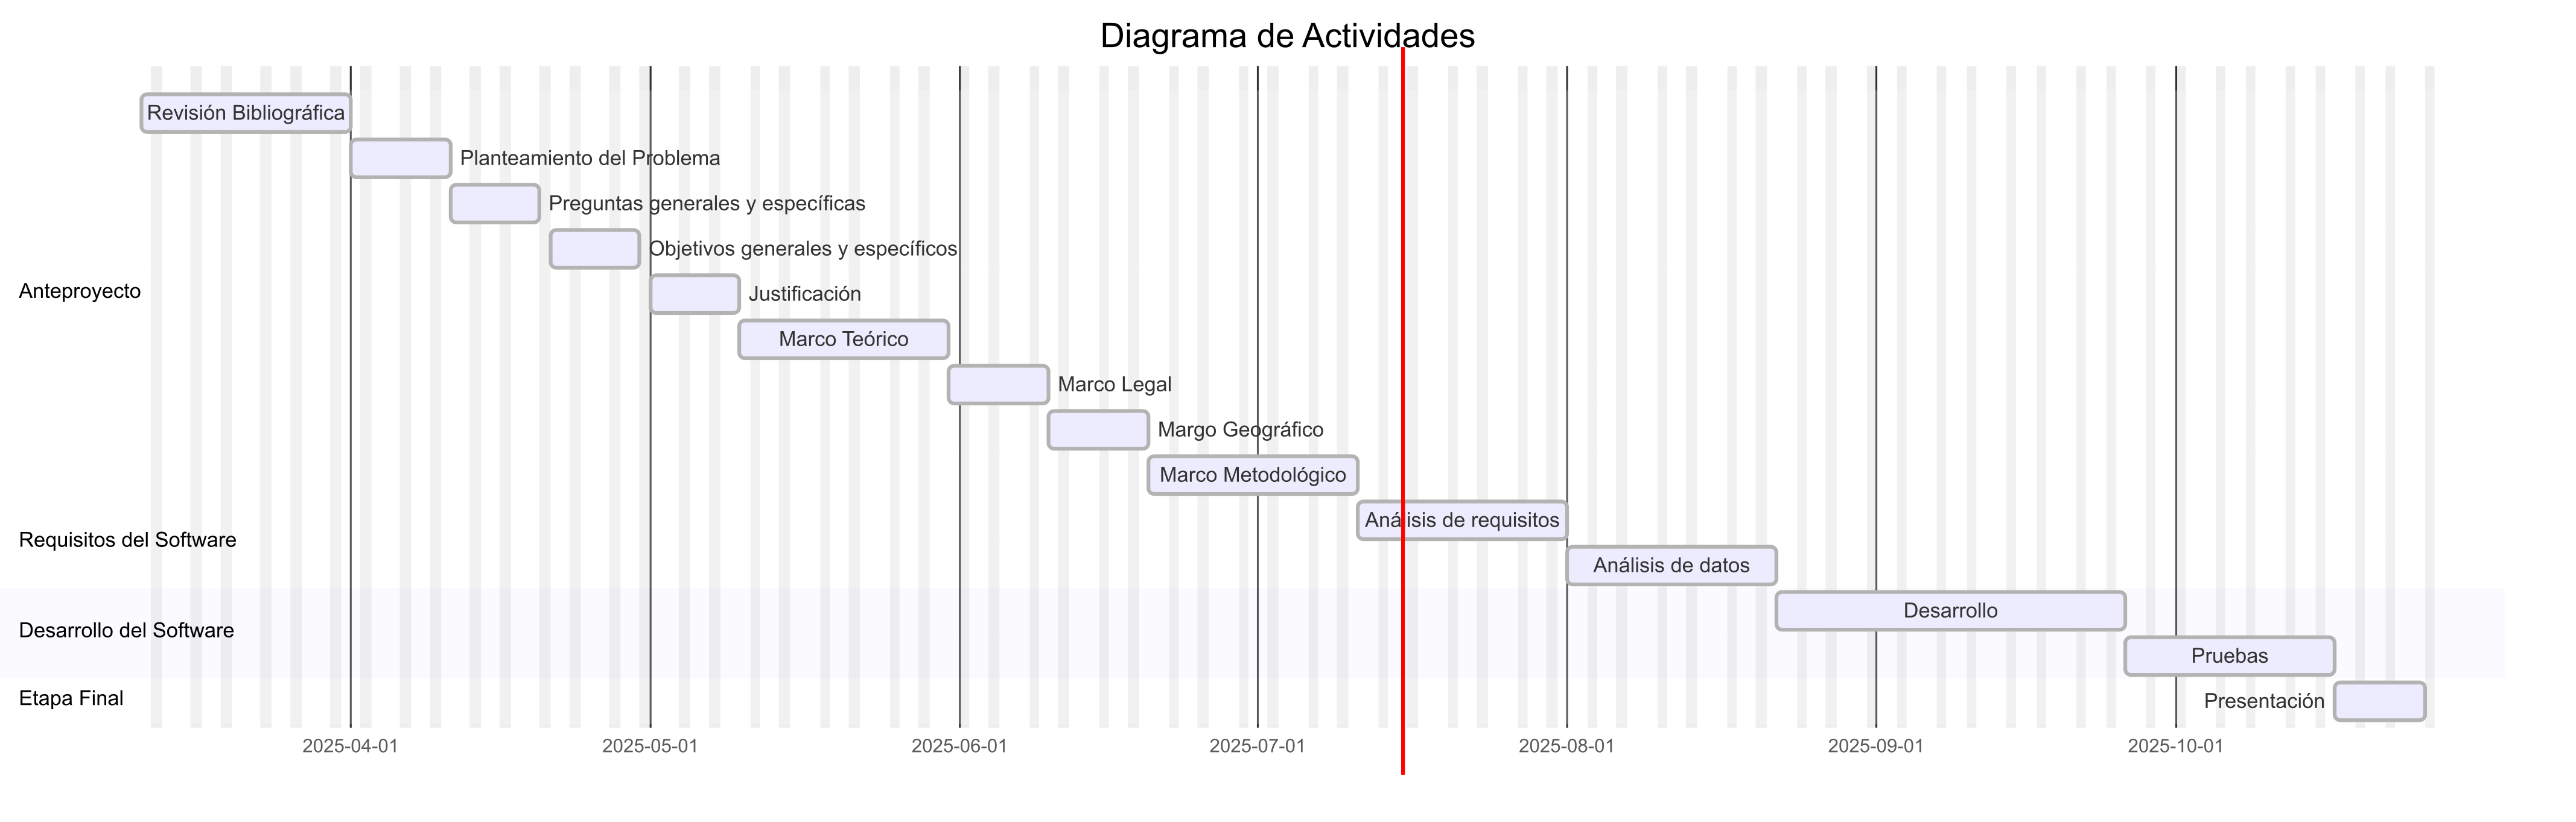
\includegraphics[width=0.85\textheight]{./img/Gantt.png}}
		\caption{Diagrama de actividades hecho con Mermaid y MarkDown.}
		\label{fig:estructura-vertical}
	\end{figure}

	\clearpage

	\section{Marco Conceptual}

	Se exponen los siguientes conceptos para el marco conceptual del trabajo. Tanto para la parte artística de las obras audiovisuales, como las partes técnicas que se usarán en el proyecto.

	\subsection{Guion Literario}

	Un guion literario es una historia desarrollada mediante imágenes, diálogos y descripciones, ubicada dentro de una estructura dramática definida. Este tipo de guión se considera la base sobre la que se construye el guion técnico y adaptativo, según \textcite{field2005} y \textcite{gulino2004}.

	\subsection{Logline}

	Según el autor \textcite{snyder2005}, un logline es un resumen breve —normalmente de una o dos frases— que presenta el conflicto central de una historia, diseñado para captar la atención del lector o espectador. Proporciona una visión clara y atractiva del núcleo narrativo del proyecto.

	\subsection{Storyline}

	Según \textcite{trottier2005}, el \textit{storyline} es la secuencia de eventos que constituyen la trama de una obra narrativa, como un libro, una película, una obra teatral, entre otros. Esta secuencia organiza las acciones de los personajes, los conflictos y sus consecuencias en una progresión estructurada que permite comprender el desarrollo de la historia.

	A diferencia de la sinopsis o del logline, que son formatos de resumen, el storyline refleja el contenido central del relato, ya que delimita cómo ocurren los hechos, en qué orden, y con qué propósito narrativo \parencite{cambridge_storyline}.

	Según el \textit{Cambridge Dictionary}, el término \textit{storyline} se refiere a la historia principal en una obra audiovisual o literaria, como una película, un libro o una obra teatral. Esta definición delimita el núcleo estructural de la narración, distinguiéndolo de elementos secundarios o subtramas.

	En este sentido, el storyline representa el hilo conductor esencial que articula el relato completo y le otorga coherencia global \parencite{cambridge_storyline}.

	\subsection{Sinopsis}

	Según \textcite{howard1995}, la \textit{sinopsis} es un resumen breve y estructurado de una obra narrativa, ya sea audiovisual o literaria, que tiene como objetivo principal captar la atención del lector, productor o evaluador del proyecto.

	Su función es presentar de manera condensada los elementos centrales de la historia —como los personajes principales, el conflicto esencial, el tono y la progresión dramática— sin desarrollar en profundidad los acontecimientos. Suele utilizarse como herramienta de venta, presentación o evaluación de guiones y proyectos creativos, y es fundamental en el contexto de pitchings o convocatorias abiertas \parencite{studiobinder_sinopsis}.

	\subsubsection{Sinopsis (según fuentes académicas y profesionales)}

	La \textit{sinopsis} es un resumen conciso que describe la trama principal de una obra narrativa, como un libro, una serie o una película. Esta descripción se elabora con el objetivo de presentar o promocionar la obra ante terceros, como productores, editores o evaluadores. A diferencia de la storyline, que detalla la progresión estructural del relato, la sinopsis se enfoca en destacar los elementos más llamativos de la historia para generar interés.

	De ahí que sea una herramienta esencial en entornos editoriales y audiovisuales, donde se requiere sintetizar la propuesta narrativa sin revelar completamente su resolución \parencite{studiobinder_sinopsis}.

	\subsection{Escaleta}

	La \textit{escaleta}, también conocida como “step outline”, es un esquema narrativo que presenta, de forma organizada, las escenas o secuencias de una obra audiovisual o literaria. Actúa como un índice de la historia, detallando brevemente lo que ocurre en cada escena (ubicación, acción principal, cambio de estado) sin incluir diálogos, lo que permite visualizar la progresión dramática y estructural de la obra \parencite{escaleta_wikipedia,aprendercine_escaleta}.

	\subsection{Escaleta (función profesional)}

	Más allá de ser un simple esquema, la escaleta es una herramienta profesional esencial para guionistas y equipos de producción. Permite ordenar sistemáticamente los bloques narrativos, identificar puntos de giro, gestionar localizaciones y distribuir tiempos, y funciona como guía para la preproducción, ya que facilita la planificación de la grabación de manera práctica y eficiente \parencite{treintaycinco_escaleta,escueladesarts_escaleta}.

	\subsection{Tratamiento}

	El \textit{tratamiento} es un relato en prosa de la historia completa, que amplía la sinopsis y escaleta, presentando cada escena como un párrafo narrativo en tiempo presente, incluyendo las acciones clave y el subtexto, pero sin diálogos técnicos. Sirve tanto para desarrollar la trama en detalle como para ofrecer un documento legible por productores y agentes literarios, con una extensión aproximada de 30 a 40 páginas en el caso de un largometraje \parencite{revista24cuadros_tratamiento,tratamiento_wikipedia}.

	\subsection{Tratamiento (paso intermedio)}

	El tratamiento es el paso narrativo intermedio entre la escaleta y el guion literario final. Se caracteriza por narrar escena por escena en prosa, incluyendo detalles narrativos y de escena, y sirve como una herramienta de planificación y visualización narrativa para garantizar coherencia en el guion final \parencite{unir_escaleta_tratamiento,tratamiento_wikipedia}.

	\subsection{Escena}

	Una \textit{escena} es la unidad narrativa que ocurre en un mismo lugar y tiempo, constituyendo la estructura básica de un guion literario o técnico. En cada escena, se presentan acciones, cambios de personajes o desarrollo dramático, representando un segmento coherente e independiente dentro del relato general \parencite{trottier_scene}.

	\subsection{Tema}

	El \textit{tema} representa el mensaje o idea central que atraviesa la obra. No suele expresarse de forma explícita en el guion, sino que está contenido en los elementos dramáticos, estructurales y emocionales de la historia. Funciona como el “ADN” del relato, conectando escenas, personajes y arcos en función de un propósito narrativo mayor \parencite{greenlight_theme,writingninja_theme}.

	\subsection{Secuencia}

	Una \textit{secuencia} es un bloque narrativo dentro de un acto que agrupa varias escenas con una mini-estructura dramática completa: inicio, desarrollo y resolución parcial. En términos audiovisuales, suelen durar entre ocho y quince minutos y funcionan como sub-relatos que mantienen la atención del espectador y avanzan la narración general \parencite{gulino_sequence,cambridge_sequence}.

	\subsection{Concepto de Ingeniería}

	Según \textcite{maida_metodologias_2015}, la ingeniería es el conjunto de conocimientos y técnicas, científicas aplicadas al desarrollo,
	implementación, mantenimiento y perfeccionamiento de estructuras (tanto físicas como teóricas)
	para la resolución de problemas que afectan la actividad cotidiana de la sociedad.

	\subsection{Concepto de Software}
	\addcontentsline{toc}{subsection}{Concepto de Ingeniería}

	Explica \textcite{maida_metodologias_2015}, el software es el equipamiento lógico e intangible de un sistema informático, que comprende el conjunto de los componentes lógicos necesarios que hacen posible la realización de tareas específicas,
	en contraposición a los componentes físicos que son llamados hardware.

	\subsection{La Importancia del Software}

	Expone \textcite{maida_metodologias_2015}, que el software es ahora la clave del éxito de muchas empresas y negocios, ya que sin él sería casi imposible el mantenimiento y crecimiento de los mismos. Lo que diferencia una compañía de otra es la suficiencia, exactitud y oportunidad de la información dada por el software.

	\subsection{Concepto de la Ingeniería de Software}

	Definen \textcite{maida_metodologias_2015}, como la disciplina o área de la informática, que hace uso razonable de los principios de ingeniería con el objetivo de obtener soluciones informáticas económicamente factible y que se adapte a las necesidades de las empresas reales, tomando en cuenta los procesos de producción y mantenimiento de software que son desarrollados y modificados en el tiempo y con los costos estimados.

	Esta ingeniería trata con áreas muy diversas de la informática y de las Ciencias de la Computación, tales como construcción de compiladores, Sistemas Operativos, o desarrollos Intranet/Internet, abordando todas las fases del ciclo de vida del desarrollo de cualquier tipo de Sistema de Información y aplicables a infinidad de áreas (negocios, investigación científica, medicina, producción, logística, banca, etc.).

	\subsection{Paradigmas del Software}

	Explican \textcite{maida_metodologias_2015}, la ingeniería de software es reconocida como una disciplina legítima, digna de tener una investigación seria, un estudio cuidadoso y generando una gran controversia.

	En la industria el ingeniero del software ha sustituido al programador como título de trabajo preferente. Los modelos de procesos de software, métodos de ingeniería de software y herramientas se han adoptado con éxito en el amplio espectro de las aplicaciones industriales.

	Un paradigma de programación es un modelo básico de diseño y desarrollo de programas, que producir programas con una directriz específica, tales como: estructura modular, fuerte cohesión, alta rentabilidad, etc.

	Continúan \textcite{maida_metodologias_2015}, existen tres categorías de paradigmas de programación:

	\begin{enumerate}[left=1.27cm]
		\item Los que soportan técnicas de programación de bajo nivel.
		\item Los que soportan métodos de diseño de algoritmos.
		\item Los que soportan soluciones de programación de alto nivel.
	\end{enumerate}

	\subsection{Análisis}

	El propósito principal, según \textcite{maida_metodologias_2015}, de esta etapa es conseguir una comprensión más precisa de los requisitos y una descripción de los mismos que sea fácil de mantener y que nos ayude a estructurar el sistema completo, incluyendo la arquitectura.

	El análisis de requerimientos facilita al ingeniero de sistemas especificar la función y comportamiento de los programas, indicar la interfaz con otros elementos del sistema y establecer las ligaduras de diseño que debe cumplir el programa.

	\subsection{Limitaciones}

	En esta etapa, según \textcite{maida_metodologias_2015}, se va a detallar la frontera del proyecto, es decir, cuál es el alcance de nuestro
	sistema.

	Todo cambio que esté fuera de las limitaciones se deberá tratar como un cambio de alcance en la
	etapa de mantenimiento.

	\subsection{Especificaciones}

	Definen \textcite{maida_metodologias_2015}, como la obtención de especificaciones a partir del cliente u otros actores intervinientes es un proceso humano muy interactivo e iterativo. Normalmente, a medida que se captura la información, se la analiza y realimenta con el cliente, refinándola, puliéndola y corrigiendo si es necesario. El analista siempre debe llegar a conocer la temática y el problema a resolver, dominarlo, hasta cierto punto, hasta el ámbito que el futuro sistema a desarrollar lo abarque.

	Al contrario de los analistas, los clientes no tiene por qué saber nada de software, ni de diseños, ni otras cosas relacionadas, sólo se debe limitar a aportar objetivos, datos e información (de mano propia	o de sus registros, equipos, empleados, etc.) al analista, y guiado por él, para que, en primera instancia defina un documento funcional y/o caso de uso.

	\subsection{Diseño y Arquitectura}

	Según \textcite{maida_metodologias_2015}, una vez realizada la etapa de análisis y especificación, se modela el sistema y definimos su estructura (incluida la arquitectura) para que soporte todos los requisitos, incluyendo los requisitos no funcionales y otras restricciones.

	Con toda esta información recopilada en los puntos anteriores, los profesionales técnicos traducen la información de alto nivel, en esquemas, diagramas, etc.\ de bajo nivel, para luego éstos ser
	comprendidos por el área de desarrollo.

	\subsection{Programación}

	Dice \textcite{maida_metodologias_2015}, que convertir un diseño a código puede ser interpretada como la parte más obvia e importante del trabajo de ingeniería de software, pero no necesariamente es la que demanda mayor trabajo y ni la más complicada. La complejidad y la duración de esta etapa está íntimamente relacionada al o a los lenguajes de programación utilizados, así también como a la calidad del diseño previamente realizado.

	\subsection{Documentación}

	Según \textcite{maida_metodologias_2015}, es la guía o comunicación escrita en sus diferentes formas, ya sea en modelaciones (UML), modelado de negocio, RUP, diagramas, pruebas, manuales de usuario, manuales técnicos, etc., todo con el propósito de eventuales correcciones, utilización, mantenimiento futuro y ampliaciones al sistema.

	La importancia de la documentación radica en que a menudo un sistema escrito por una persona es modificado por otra. Es por ello que la documentación sirve para facilitar la etapa de mantenimiento.

	La documentación se compone de tres partes:

	\begin{itemize}[label=\textbullet, leftmargin=1.27cm]
		\item \textbf{Documentación Interna}: Son los comentarios o mensajes que se añaden al código fuente para hacer más claro el entendimiento de los procesos que lo conforman, incluyendo las precondiciones y las postcondiciones de cada función.
		\item \textbf{Documentación Externa}: se define en un documento escrito con los siguientes puntos:
			\begin{itemize}[label=○]
				\item Descripción del Problema
				\item Datos del Autor
				\item Algoritmo (diagrama de flujo o Pseudocódigo)
				\item Diccionario de Datos
				\item Código Fuente (programa)
			\end{itemize}
		\item \textbf{Manual de Usuario}: Describe paso a paso la manera cómo funciona el programa, con el fin de que el usuario lo pueda manejar para que obtenga el resultado deseado.
	\end{itemize}

	\subsection{Mantenimiento}

	Coincide \textcite{maida_metodologias_2015}, que el mantenimiento consiste en mantener y mejorar el software para enfrentar errores descubiertos y nuevos requisitos. Esto puede llevar más tiempo incluso que el desarrollo inicial del software.

	La fase de mantenimiento de software es una parte explícita del modelo en cascada del proceso de desarrollo de software el cual fue desarrollado durante el movimiento de programación estructurada en computadores. El otro gran modelo, el Desarrollo en espiral desarrollado durante el movimiento de ingeniería de software orientada a objeto no hace una mención explícita de la fase de mantenimiento.

	En un ambiente formal de desarrollo de software, la organización o equipo de desarrollo tendrán algún mecanismo para documentar y rastrear defectos y deficiencias. El Software tan igual como la mayoría de otros productos, es típicamente lanzado con un conjunto conocido de defectos y deficiencias.

	\subsection{Contenedores}

	Según lo describe \textcite{merkel2014}, los contenedores son entornos aislados a nivel de sistema operativo que permiten empaquetar y ejecutar aplicaciones junto con todas sus dependencias. Esta tecnología permite asegurar la portabilidad del software, ya que puede ejecutarse de forma consistente en cualquier entorno que tenga un motor de contenedores.

	A diferencia de las máquinas virtuales tradicionales, los contenedores comparten el núcleo del sistema operativo, lo que los hace más livianos y eficientes en recursos.

	\subsection{Podman}

	Según \textcite{redhat2021}, \textit{Podman} es una herramienta de gestión de contenedores compatible con OCI (\textit{Open Container Initiative}), que permite crear, ejecutar y mantener contenedores sin necesidad de un demonio centralizado como ocurre en \textit{Docker}.

	Se distingue por su enfoque en la seguridad, ya que permite la ejecución como usuario sin privilegios, lo que lo hace adecuado para entornos de desarrollo y producción con altos estándares de control de acceso.

	\subsection{Podman Desktop}

	\textit{Podman Desktop} es una herramienta gráfica de código abierto y multiplataforma desarrollada por Red-Hat (contribución comunitaria), diseñada para simplificar la gestión de contenedores y flujos de trabajo de Kubernetes en entornos locales. Proporciona un entorno visual para crear, ejecutar, inspeccionar y depurar contenedores y pods, además de permitir construir YAML de Kubernetes y probar despliegues locales \parencite{redhat_podman_desktop,georger2024}.

	Además, ofrece compatibilidad con múltiples motores (Podman, Docker, CRC, Lima), integrándose bien con herramientas OCI y APIs de Docker \parencite{podman_desktop_multi}.

	\subsection{API (Interfaz de programación de aplicaciones)}

	Una API (por sus siglas en inglés, \emph{Application Programming Interface}) es un conjunto de reglas y protocolos que permiten la comunicación entre componentes de software, facilitando el intercambio de datos y funcionalidades mediante solicitudes y respuestas estructuradas \parencite{aws_api,oracle_api}.

	En contraste con una interfaz de usuario, la API conecta programas o sistemas, incluidos servicios web, bibliotecas y sistemas operativos \parencite{wikipedia_api}.

	\subsection{Kanban}

	El término \emph{Kanban} (del japonés “letrero” o “tarjeta”) describe tanto un sistema de señales para gestión de inventarios bajo producción justo a tiempo, como un método ágil para la gestión visual del trabajo.

	Utilizado originalmente en Toyota, se basa en tarjetas o tableros que indican cuándo comenzar o detener tareas, limitando el trabajo en curso y mejorando la eficiencia \parencite{wikipedia_kanban_dev,asana_kanban}.

	\subsection{Entorno de Desarrollo Integrado (IDE)}

	Un IDE (\emph{Integrated Development Environment}) es una aplicación que integra en una sola interfaz el editor de código, herramientas de compilación, depuración y, a menudo, control de versiones, con el fin de mejorar la productividad de los desarrolladores \parencite{eswiki_ide,geeksforgeeks_ide}.

	Proporciona funciones como resaltado de sintaxis, auto-completado, inspección de clases y manejo de proyectos, todo accesible desde una sola ventana \parencite{eswiki_ide}.

	\section{Marco Histórico}

	Antes de la redacción del guion literario, existió una evolución histórica significativa en la creación de estructuras narrativas audiovisuales, que respondieron a necesidades técnicas, económicas y artesanales del cine.

	\subsection{El cine mudo y los guiones de continuidad}

	Durante la era del cine mudo (finales del siglo XIX a fines de los años 1920), las herramientas para organizar la narrativa eran rudimentarias. Los primeros guiones, llamados «continuity scripts» o escenarios, consistían en listados de escenas, con breves descripciones de acciones visuales y planos, diseñados para evitar improvisaciones en rodaje y reducir costos de producción \parencite{screenplayology_history}.

	\subsection{Nacimiento del guion literario}

	Con el advenimiento del sonido, los guiones evolucionaron para incluir diálogos y descripciones más detalladas, consolidándose en una forma escrita que combinaba estructura visual y verbal. El sistema de tres actos, promovido por Syd Field desde 1979, se convirtió en un paradigma ampliamente adoptado en Hollywood, con puntos de giro claramente definidos para guiar el desarrollo dramático \parencite{newyorker_mckee,newyorker_mckee2}.

	\subsection{Origen del storyboard y la preproducción gráfica}

	En la década de 1930, estudios como Disney popularizaron el uso de la \textbf{escaleta visual} o \textit{storyboard}, un paso clave antes del guion literario. Esta técnica permitió visualizar escenas enteras con dibujos, facilitando la planificación visual y de producción \parencite{storyboard_wikipedia}.

	\subsection{Consolidación del guion literario}

	A partir de los 1940--50, la transición técnica y académica del guion continuó con manuales profesionales como los de Field y McKee. Estas obras definieron estándares narrativos y formales que siguen siendo referencia para la planificación narrativa en cine y televisión \parencite{screenplayology_history,newyorker_mckee}.

	\subsection{Primeros guiones: escenarios y continuity scripts}
	En los inicios del cine mudo (finales del siglo XIX hasta finales de los años 1920), los guiones eran conocidos como «scenario» o \textit{continuity scripts}. Estos consistían en listados de escenas que describían acciones visuales y ángulos de cámara, creados para organizar la producción sin depender de improvisaciones sobre el set, lo que representó un avance lógico frente a las ineficiencias en costos y tiempos de rodaje \parencite{thescriptlab_history,screenplayology_history,wcftr_continuity}.

	\subsection{Nacimiento del guion literario y estructura narrativa}
	La incorporación del sonido en 1927 provocó que los guionistas añadieran diálogos y descripciones más complejas, consolidando así el guion literario con una estructura dramática más consciente.

	Desde finales de los años 1930 y consolidado en los 1940–50, Syd Field propuso un modelo de tres actos con puntos de giro bien definidos —una base narrativa adoptada por la industria— mientras autores como Robert McKee profundizaron el análisis de elementos como la \textit{storyline}, el \textit{logline}, el \textit{tema}, las \textit{escenas} y \textit{secuencias} para comprender integralmente la trama, \parencite{screenwriting_history_scriptor, thescriptlab_history}

	\subsection{Historia del storyboard y su rol en la preproducción}
	En la década de 1930, \textit{Walt Disney} y su equipo introdujeron el storyboard, antecedente visual directo del guion técnico, mediante dibujos secuenciales que permitían anticipar escenas y organizar la producción. Atribuido a Webb Smith en Disney y usado por primera vez para cortos animados como \textit{Three Little Pigs} (1933), el storyboard se consolidó como herramienta de preproducción en estudios globales \parencite{thescriptlab_history}.

	\subsection{Evolución posterior: long-form y transmedia}
	Desde los años 1970 en adelante, surgieron formatos como guiones por especulación (\textit{spec scripts}) y herramientas narrativas más refinadas —loglines, beat sheets, tratamientos— para desarrollar proyectos transmedia, series y cine independiente. Los guiones avanzaron hacia una clara definición de \textit{secuelas}, \textit{escenas} y \textit{tema}, así como una narrativa visual coherente desde etapas iniciales de preproducción, \parencite{thescriptlab_history}

	\subsection{Primeras herramientas de formato automatizado}
	En los años 1980, surgieron los primeros software de formateo de guiones, como \textit{Scriptor} (1983), que automatizaban la conversión de texto plano en guiones con formato profesional, marcando la transición desde el procesamiento manual a herramientas digitales especializadas \parencite{screenwriting_history_scriptor}.

	\subsection{Dominio del software comercial}
	{\sloppy
		Entre 1990 y 2000, herramientas como \textit{Final Draft} (1990) y \textit{Movie Magic Screenwriter} se consolidaron como estándares de la industria, ofreciendo formatos robustos, gestión de versiones y herramientas de producción. \textit{Final Draft} recibió en 2013 el premio Emmy por su innovación tecnológica \parencite{turn0search22FinalDraft,turn0search27MovieMagic}.
	}

	\subsection{Alternativas asequibles y emergentes}
	{\sloppy
		En la década del 2000 surgieron alternativas accesibles, como \textit{Celtx} \parencite{turn0search23Celtx} que al inicio fue software libre de escritorio y luego un servicio web con funcionalidades de guion, storyboard y producción, basado en estándares abiertos como XML y RDF\@.

		También apareció \textit{Fade In} (2008), \parencite{turn0search22FinalDraft} una opción comercial con costo reducido (\ensuremath{\sim\$80} USD), elogiada por su interfaz limpia y compatibilidad con formatos profesionales.
	}

	\subsection{Software colaborativo y en la nube}
	Desde 2013, \textit{WriterDuet} \parencite{turn0search24WriterDuet} revolucionó la colaboración remota en tiempo real, usando la nube para sincronización de guiones, edición conjunta y respaldo automático, ganando popularidad rápidamente.

	\subsection{Herramientas libres y Open Source}
	En el entorno libre destacan \textit{Trelby} (basado en \textit{Blyte}, abierto al GPL desde 2006) y \textit{Kit Scenarist}, ambos gratuitos y compatibles con formatos comunes, ofreciendo autocompletado, organización de escenas y exportación a FDX/PDF/Fountain \parencite{turn0search21Trelby} y \parencite{turn0search11KitScenarist}. Además, \textit{Story Architect} (Starc) en GitHub es una evolución de Kit Scenarist enfocada a la narración extensiva \parencite{turn0search17StoryArchitect}

	\subsection{Software especializado para preproducción}
	Programas como \textit{Genie Workbench} (2009) ofrecen herramientas modulares para planificación de filmación (schedule, cast, crew), siendo open source bajo licencia BSD, y generando automatización de workflows en etapas previas al guion literario \parencite{turn0search26GenieWorkbench}.

	\subsection{Evolución del Formato Abierto Fountain}

	A lo largo de la historia de la escritura de guiones, la industria audiovisual ha estado condicionada por formatos propietarios y entornos cerrados de edición. Desde finales del siglo XX, el uso de programas como \textit{Final Draft}, \textit{Movie Magic Screenwriter} y \textit{Celtx} estableció una dependencia casi obligatoria de formatos como FDX o documentos enriquecidos con esquemas binarios, los cuales limitaban la portabilidad y archivabilidad de los guiones. Esta situación originó múltiples dificultades para escritores independientes, desarrolladores de software, archivistas y académicos que buscaban mantener acceso abierto y control sobre sus obras \parencite{fountain_wikipedia}.

	El problema se agravó con el auge de las plataformas basadas en la nube, donde los guionistas comenzaron a depender aún más de infraestructuras externas para almacenar y editar sus obras. Esta dependencia tecnológica incentivó la búsqueda de soluciones abiertas, interoperables y sostenibles en el tiempo, que permitieran mantener la integridad narrativa de los guiones sin sacrificar su portabilidad. En este contexto nació \textit{Fountain}.

	Fountain fue creado en 2012 por John August, Stu Maschwitz y Nima Yousefi, como una solución simple pero poderosa: usar texto plano para escribir guiones respetando convenciones narrativas clásicas. Su objetivo fue permitir que cualquier persona pudiera escribir un guion completo en un editor de texto básico, como \texttt{vim}, \texttt{Notepad++}, o incluso desde el navegador, sin requerir software privativo ni estructura binaria. El formato reconoce elementos comunes del guion —como encabezados de escena, acciones, diálogos y transiciones— mediante convenciones legibles, eliminando así la barrera entre el contenido narrativo y la forma técnica \parencite{fountain_official}.

	El estándar Fountain representa una transformación dentro de la práctica del guionismo moderno, ya que rompe con décadas de opacidad en los formatos y devuelve el control al autor. Además, su adopción en herramientas como Trelby, Kit Scenarist, Fade In, Slugline y múltiples librerías en Python, JavaScript y Rust, lo ha convertido en una pieza fundamental para la interoperabilidad entre plataformas de software de escritura profesional y herramientas libres \parencite{fountain_github, nofilmschool_fountain}.

	En el contexto del presente estudio, Fountain tiene relevancia no solo por su rol funcional en la escritura de guiones, sino también por su dimensión política y tecnológica como formato de preservación, archivo y autonomía creativa. Representa una respuesta directa a las limitaciones impuestas por décadas de formatos propietarios, al mismo tiempo que ofrece un modelo reproducible para nuevas herramientas digitales como \textit{DREAMINK}.

	\section{Marco Legal}

	El marco legal aplicado al uso de software y la creación de guiones literarios en Paraguay abarca normativas internacionales y locales que protegen la propiedad intelectual y establecen derechos sobre obras audiovisuales, estructuras pre-guion literario y programas informáticos.

	\subsection{Tratados internacionales}

	Paraguay es signatario de los principales convenios internacionales sobre derechos de autor, entre ellos el \textbf{Convenio de Berna} (1886), que establece la protección automática de obras literarias y artísticas desde su fijación en un medio fijo \parencite{berne2025,rule_shorter_term}.

	También se adhiere al \textbf{Tratado de Beijing sobre Actuaciones Audiovisuales} (2012), orientado a proteger derechos de intérpretes y fortalecer la regulación legal de obras audiovisuales \parencite{beijing_treaty2025}.

	\subsection{Protección de software y guiones}

	{\sloppy
		El \textbf{Derecho de Autor} paraguayo reconoce la creación intelectual, incluyendo software y guiones literarios, a través de la Ley 1328/1998, modificada por la Ley 4046/2010. Esta normativa ampara tanto los derechos económicos como morales de los autores, sin exigir registro previo \parencite{wipo_paraguay}.
	}

	Los programas informáticos están cubiertos como obras literarias, lo que incluye tanto su código como su interfaz gráfica \parencite{njq_paraguay,paraguay_software1998}.

	\subsection{Aplicabilidad a estructuras pre-guion literario}

	El Convenio de Berna extiende la protección a «obras literarias», abarcando guiones literarios, \textit{storylines}, escaletas y tratamientos, siempre que se encuentren fijados en un medio tangible, lo que incluye documentos digitales \parencite{berne2025}.

	En cuanto al software especializado para preproducción (por ejemplo, generadores de \textit{storyboards}), la ley cubre la protección de su código fuente y compilado, aunque los datos o estructuras generadas (ej.\ escaletas) pueden requerir protección adicional bajo derechos conexos o contratos.

	\subsection{Gestión colectiva y cumplimiento local}

	En Paraguay, los autores pueden inscribirse en \textbf{Autores Paraguayos Asociados (APA)}, entidad de gestión colectiva creada en 1951 y regulada por la Ley 1328/1998, para administrar sus derechos económicos en el territorio nacional e internacional \parencite{apa_py}.

	En paralelo, la aplicación de la legislación local está a cargo de la \textbf{Dirección Nacional de Propiedad Intelectual (DINAPI)}, que regula infracciones y sanciones ante violaciones del derecho de autor \parencite{ip_office_py}.

	\subsection{Fountain como Estándar Abierto}

	\textit{Fountain} es un lenguaje de marcado de texto plano y de código abierto diseñado para la creación y edición de guiones en cualquier editor de texto, independientemente del sistema operativo o la plataforma. Fue desarrollado por Stu Maschwitz, John August y Nima Yousefi, entre otros colaboradores, con el objetivo de facilitar la escritura y el intercambio de guiones sin restricciones de formato propietarios \parencite{fountain_wikipedia, fountain_official}.

	Desde su lanzamiento, \textit{Fountain} se ha consolidado como una alternativa viable a los formatos propietarios (como FDX de Final Draft), promoviendo la accesibilidad y portabilidad. Su especificación y múltiples librerías de código abierto están disponibles bajo licencia MIT, lo que permite su integración en aplicaciones de edición, conversión y archivado sin preocuparse por la obsolescencia del software \parencite{fountain_official, fountain_github}.

	Legalmente, \textit{Fountain} representa un enfoque innovador hacia el software y estándares abiertos, en donde el formato de guion se define en un documento legible y libremente distribuible. Esto permite que los guionistas mantengan \textit{control y propiedad total} de sus creaciones sin depender de licencias restrictivas ni formatos propietarios, alineándose con las prácticas recomendadas de preservación digital y acceso abierto.

	\section{Marco Geográfico}

	El presente proyecto, titulado \textit{DREAMINK}, se enmarca dentro de un enfoque geográfico no convencional, dado que no se restringe a un espacio físico cerrado ni a una institución específica, sino que está orientado a la comunidad global de guionistas, narradores visuales y desarrolladores de contenido audiovisual.

	Desde una perspectiva territorial, la iniciativa nace en Paraguay, como parte de un trabajo de grado desarrollado por estudiantes de la carrera de Técnico Superior en Programación de Aplicaciones Informáticas. Sin embargo, el alcance de la aplicación es universal, ya que se trata de un \textit{software libre y de código abierto} que será distribuido públicamente a través de un repositorio remoto (\textit{Codeberg}), disponible para cualquier persona con acceso a internet, sin distinción de ubicación geográfica o afiliación institucional.

	En cuanto al espacio social y cultural, el sistema está dirigido especialmente a guionistas independientes, pequeños estudios de producción, colectivos artísticos, docentes de narrativa audiovisual y estudiantes de cine y guion, tanto de Paraguay como del resto del mundo hispanohablante. Este grupo objetivo comparte características comunes como la necesidad de herramientas accesibles, funcionales y estandarizadas para organizar sus proyectos creativos antes de la redacción del guion literario.

	\textit{DREAMINK} también se sitúa institucionalmente dentro del paradigma del software libre, promoviendo valores como la cooperación, la transparencia, la documentación abierta y la soberanía tecnológica. Al ser alojado en una plataforma abierta, el sistema puede ser replicado, auditado, traducido y adaptado a distintas realidades locales, manteniendo su independencia respecto a proveedores o empresas específicas.

	Por lo tanto, el presente proyecto se sitúa en una doble dimensión geográfica: por un lado, como una producción académica paraguaya con características regionales específicas; y por otro lado, como una herramienta global orientada a una comunidad transnacional de creadores audiovisuales que comparten la necesidad de estructurar sus obras de manera eficiente y libre.

	\section{Marco Metodológico}

	\subsection{M\'etodo de la investigaci\'on}

	El presente estudio emplea un m\'etodo de investigaci\'on \textbf{básico}, dado que tiene como objetivo el desarrollo de una herramienta tecnol\'ogica orientada a resolver un problema concreto identificado en el proceso de pre--escritura de guiones audiovisuales, particularmente en la etapa de estructuraci\'on narrativa.

	Según la profundidad, puede ser \textbf{descriptiva} al ser dirigidos a determinar cómo es y cómo está la forma actual de realizar una etapa de estructuraci\'on narrativa previa al guion literario.

	El método que fue utilizado era la observación participativa y el apoyo de las entrevistas, análisis del problema y los contenidos, así como también la observación.

	El alcance temporal de diseño tipo transversal (porque el estudio se realiza en un solo periodo), entre los meses de febrero a noviembre del año 2025.

	\subsection{Diseño de la Investigación}

	El diseño de la investigación es \textbf{experimental}, porque se realiza previo a los datos a ser recolectados mediante encuestas y las pruebas de uso de la aplicación.

	\subsection{Enfoque}

	El estudio se encuentra dentro del enfoque mixto, porque se pueden utilizar los tipos de datos cuantitativos y cualitativos.

	\subsection{Nivel de la Investigación}

	El nivel de la investigación es de tipo \textbf{explicativo}, porque nos enfocaremos en conocer los problemas que rodean a la investigación y de allí partir a desarrollar una solución.

	\subsection{Universo de la Investigación}

	El universo de la investigación es para diferentes guionistas paraguayos elegidos de manera aleatoria, que se dediquen explícitamente al cine dentro de la República del Paraguay.

	\subsection{Población}

	La población va a ser para los guionistas paraguayos que serán elegidos de manera aleatoria dentro de la República del Paraguay.

	\subsection{Muestra}

	La muestra será la población de esos guionistas paraguayos elegidos de manera aleatoria.

	\subsection{Instrumento de Recolección de Datos}

	El instrumento de recolección de datos será utilizado las encuestas y las observaciones, sobre las encuestas se puede usar preguntas cerradas para obtener la información de la población.

	\subsection{Técnica de Análisis de los Datos}

	La técnica de análisis de los datos que se podrán usar es la cuantitativa y la cualitativa, y todos los datos serán procesados de manera gráfica y el uso de formularios electrónicos.

	\printbibliography{}

\end{document}
